\noindent

\includegraphics[height=1.25cm]{images/pictograms/replication}

\includegraphics[height=1.25cm]{images/pictograms/under_construction}

\includegraphics[height=1.25cm]{images/pictograms/bsc}

%%%%%%%%%%%%%%%%%%%%%%%%%%%%%%%%%%%%%%%%%%%%%%%%%%%%%%%%%%%%%%%%%%%%%%%%%%%%%%%%%%%%%%%%%%%%%%%%%%%

\begin{flushright} {\tiny {\color{gray} python\_codes/fieldstone\_183/text.tex}} \end{flushright}

\par\noindent\rule{\textwidth}{0.4pt}

\begin{center}
\inpython
{\small Code: \url{https://github.com/cedrict/fieldstone/tree/master/python_codes/fieldstone_183}}
\end{center}

\par\noindent\rule{\textwidth}{0.4pt}

{\sl This stone was developed in collaboration with A. van Meegdenburg and Sylas van der Biezen.}.

\par\noindent\rule{\textwidth}{0.4pt}

Last revision: May. 1st, 2026.

\par\noindent\rule{\textwidth}{0.4pt}

%%%%%%%%%%%%%%%%%%%%%%%%%%%%%%%%%%%%%%%%%%%%%%%%%%%%%%%%%%%%%%%%%%%%%%%%%%%%%%%%%%%%%%%%%%%%%%%%%%%

The rationale behind this \stone is that replicating articles showcasing whole planets 
has us rely on the equations in the text for the density, the viscosity and the initial 
temperature. It then makes sense to first create a 1d profile of the planet and thereby
verify that the equations in the text are valid. As we will see, not always the case. 

%%%%%%%%%%%%%%%%%%%%%%%%%%%%%%%%%%%%%%
\section*{Mars a la King et al}

We shall here study 3 articles:

\begin{itemize}
\item \fullcite{rozh06}
\item \fullcite{seki14}
\item \fullcite{muki24}
\end{itemize}

%-------------------------------
\subsection*{\textcite{muki24}}

We start by defining all the required parameters (see {\tt stone\_muki24.py}):

\begin{lstlisting}
Rsurf=3.3895e6
Rcmb=1.830e6
rho0=3500
g=3.72
eta0=1e21
V=6.6e-6
alpha=2e-5
kappa=1e-6
hcapa=1250
Tsurf=220
DeltaT=1500
Tm=1720
\end{lstlisting}

Note that we will be exploring 2 values of $E_a$, 3 values of $T_{cmb}$ and 3 coefficients in front of $\Delta T$.

We then proceed to build a 1d mesh, with $R_{cmb} < r < R_{surf}$:

\begin{lstlisting}
dr=(Rsurf-Rcmb)/(npts-1) 
r=np.zeros(npts,dtype=np.float64)
for i in range(0,npts):
    r[i]=Rcmb+dr*i
\end{lstlisting}

Turning now to the initial temperature profile we quickly realise that 
Eqs. (10,11) of the paper are wrong. They should contain $\kappa$ under 
the square root, and there seems to be a confusion between $T_m$, $T_{surf}$ 
and $T_{cmb}$ in some places. 
Instead we rely on the following function which serves the same purpose:
\begin{lstlisting}
def initial_temperature_hsc(r,Rcmb,Rsurf,Tcmb,Tsurf,age_cmb,age_surf,Tm,kappa):
    val=Tsurf+(Tm-Tsurf)*special.erf((Rsurf-r)/2/np.sqrt(age_surf*kappa))\
             -(Tcmb-Tm)*(-1+special.erf((r-Rcmb)/2/np.sqrt(age_cmb*kappa)))
    return val
\end{lstlisting}
which we then use as follows:
\begin{lstlisting}
Tcmb=Tsurf+coeff*DeltaT
T=np.zeros(npts,dtype=np.float64)
for i in range(0,npts):
    T[i]=initial_temperature_hsc(r[i],Rcmb,Rsurf,Tcmb,Tsurf,age_cmb,age_surf,Tm,kappa)
\end{lstlisting}

We can then vary $T_{cmb}$ (via the 3 different values of $\Delta T$) and the age
of the half-space cooling model:
\begin{center}
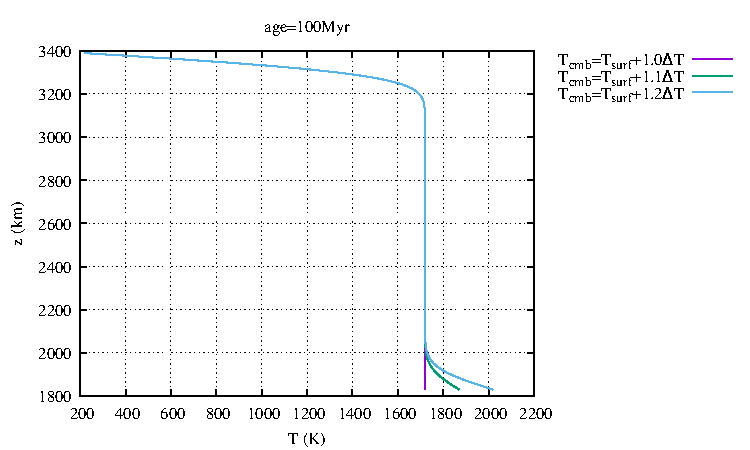
\includegraphics[width=5.7cm]{python_codes/fieldstone_183/muki24/T100.pdf}
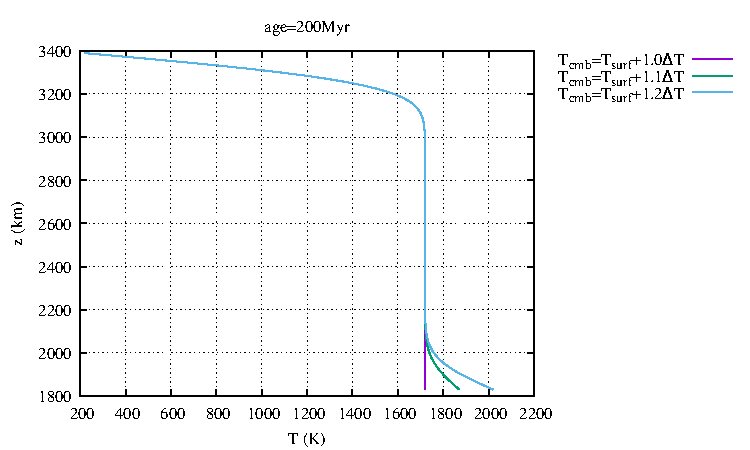
\includegraphics[width=5.7cm]{python_codes/fieldstone_183/muki24/T200.pdf}
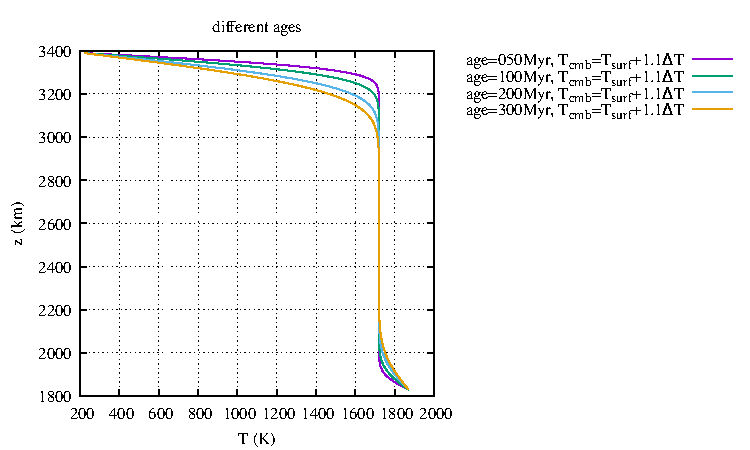
\includegraphics[width=5.7cm]{python_codes/fieldstone_183/muki24/T123.pdf}
\end{center}

We can then compute the corresponding density and the pressure profiles:
\begin{lstlisting}
rho=np.zeros(npts,dtype=np.float64)
for i in range(0,npts):
    rho[i]=rho0*(1-alpha*T[i])

p=np.zeros(npts,dtype=np.float64)
p[npts-1]=0
for i in range(npts-2,-1,-1):
    p[i]=p[i+1]+(rho[i]+rho[i+1])/2*g*dr
\end{lstlisting}

\begin{center}
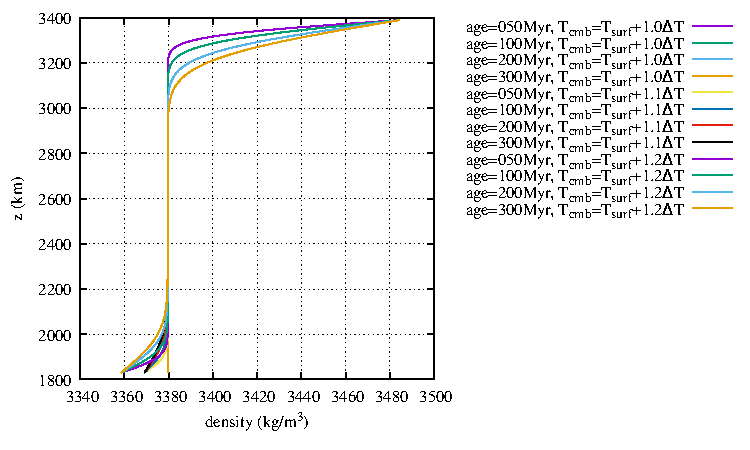
\includegraphics[width=8cm]{python_codes/fieldstone_183/muki24/rho.pdf}
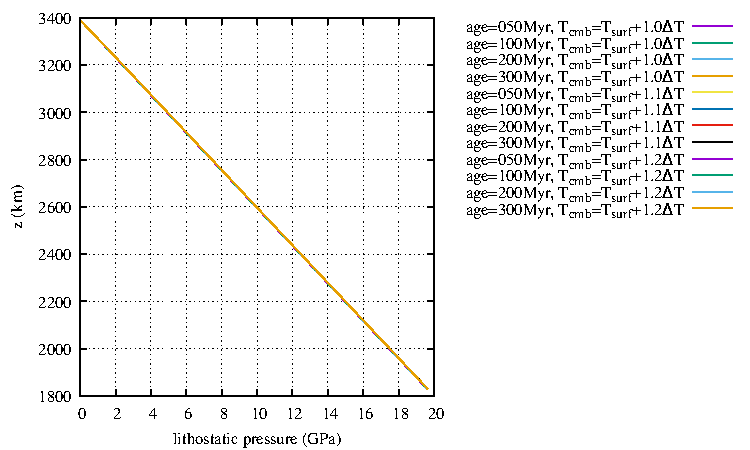
\includegraphics[width=8cm]{python_codes/fieldstone_183/muki24/p.pdf}
\end{center}



In section 2.3.1 we read:
\begin{displayquote}{\color{darkgray}
Based on Christensen and Yuen (1984), activation energy is divided by 
the stress exponent $n$ to approximate a power law rheology for olivine. 
Typically $n$ is taken to be 3, but we vary the effective activation energy, 
corresponding to testing values of $n=3$ (dislocation creep) and $n=1$ 
(diffusion creep). Thus to approximate $n=3$, the nominal activation energy of
$350 kJ/mol$ becomes $117 kJ/mol$ (low activation energy cases), while 
for $n=1$, we keep the activation as $350 kJ/mol$ (high activation energy cases).

The temperature and pressure (depth) dependent viscosity $\eta$ is given, 
in dimensional form, by
\[
\eta = A \eta_0 \exp \left( \frac{E_a + p V_a}{RT} 
-\frac{E_a + p V_a}{R(\Delta T + T_s)}  \right)
\]
where $\eta_0$ is the reference viscosity ($10^{21}$ Pa s), $E_a$ is the 
activation energy (either 117 or 350 kJ/mol), $p$ is the pressure, $V_a$ is 
the activation volume (6.6 cm3/mol), $R$ is the ideal gas constant, and $T$ 
is the potential temperature (in K). The pre‐exponential factor $A$ is to 
control the viscosity by layer. To enforce a strong (initially 100 km thick) 
lithosphere, from the surface to 100 km depth, $A=10$. From 100 to 1,000 km 
depth, $A=0.1$, establishing a weak martian upper mantle rheology. 
From 1,000 km depth to the CMB, $A=10$, accounting for a strong lower martian 
mantle rheology.}
\end{displayquote}

This translates as follows (a maximum viscosity cutoff has been implemented):

\begin{lstlisting}
eta=np.zeros(npts,dtype=np.float64)
for i in range(0,npts):
    depth=Rsurf-r[i]
    if depth<100e3: 
       A=10
    elif depth<1000e3:
       A=0.1
    else: 
       A=10
    eta[i]=A*eta0*np.exp((E+p[i]*V)/R/T[i]-(E+p[i]*V)/R/(DeltaT+Tsurf))
    eta[i]=min(eta[i],1e25) 
\end{lstlisting}

Since $V_a$, $\Delta T$ and $T_{surf}$ are kept constant, the viscosity only depends 
on $p,T$ and $E$:

\begin{center}
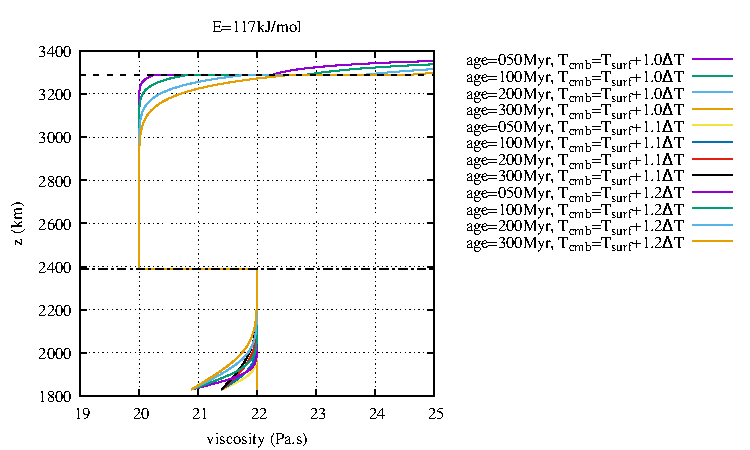
\includegraphics[width=8cm]{python_codes/fieldstone_183/muki24/eta_E117.pdf}
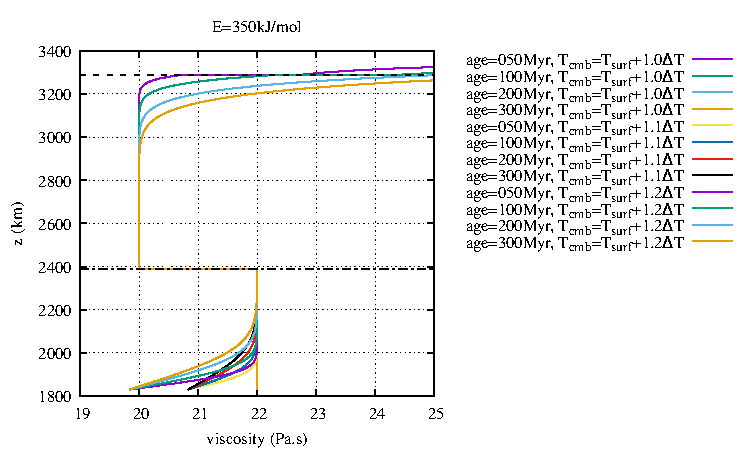
\includegraphics[width=8cm]{python_codes/fieldstone_183/muki24/eta_E350.pdf}
\end{center}

In practice the viscosity formulation above is not very common and 
might be somewhat problematic to implement in existing codes.
However, this can be easily remedied as follows: 
If one replaces the pressure by the lithostatic pressure in the second 
term inside the exponential, then the entire second term is then 
function of the vertical coordinate only and can then be 'merged' into 
the $A$ term:
\begin{eqnarray}
\eta 
&=& A(z) \eta_0 \exp \left( \frac{E_a + p V_a}{RT} 
-\frac{E_a + p V_a}{R(\Delta T + T_s)}  \right) \nn\\
&\simeq& A(z) \eta_0 \exp \left( \frac{E_a + p V_a}{RT} 
-\frac{E_a + p_L(z) V_a}{R(\Delta T + T_s)}  \right) \nn\\
&=& A(z) \eta_0 \exp \left( \frac{E_a + p V_a}{RT} \right) 
\left(-\frac{E_a + p_L(z) V_a}{R(\Delta T + T_s)}  \right) \nn\\
&=& \eta_0 \underbrace{A(z) \left(-\frac{E_a + p_L(z) V_a}
{R(\Delta T + T_s)}  \right)}_{A'(z)}
\exp \left( \frac{E_a + p V_a}{RT} \right) 
\end{eqnarray}
This expression is then akin to a diffusion creep viscosity
albeit with a depth dependent prefactor. 
 


%-------------------------------
\subsection*{\textcite{seki14}}

Important information taken from the paper: 
``Boussinesq approximation'', ``We do not have a compositionally distinct crust.''.

We also read ``The calculations are performed in a 3D spherical shell
with a free-slip cold upper boundary and a stress-free core–mantle
boundary.'' I do not understand this, how is a stress-free cmb different than
free slip surface?

The initial temperature is specified as follows:
``
The calculations begin with a conductive boundary layer
at the surface and an initial non-dimensional mantle temperature
of 0.95 with an error function temperature profile for the top ther-
mal boundary layer (250 Myr).''

``We fix the surface temperature at 220 K while the core-mantle boundary 
is at 1820 K at a depth of 1780 km. [...] The
initial temperature difference across the mantle is 1600 K.''


``We consider a Newtonian rheology with a strong temperature-
dependent viscosity and a layered viscosity structure that includes
a viscosity increase by a factor of 8 and 25 at a depth of 996 km \cite{rozh06}.''
Eq. 6 in the paper is written in dimensionless form, mixing primed and 
not primed quantities, but Eq 7 allows us to arrive at the conclusion 
that it is the same form as in \cite{muki24} above, although the
radial dependency $\eta(r)$ is not specified.
I then implemented this for simplicity:
\begin{lstlisting}
if depth<996e3: 
   A=1
else: 
   A=8
eta[i]=A*eta0*np.exp((E+p[i]*V)/R/T[i]-(E+p[i]*V)/R/(DeltaT+Tsurf))
\end{lstlisting}



We find most of these parameters in table 1 of the paper (see {\tt stone\_seki14.py}):
\begin{lstlisting}
Rsurf=3.398e6
Rcmb=Rsurf-1780e3 
rho0=3400
g=3.72
eta0=1e21
R=8.314
V=3.61e-6
alpha=3e-5
kappa=1e-6
hcapa=1200
Tsurf=220
DeltaT=1600
E=157e3 
Tcmb=Tsurf+DeltaT
Tm=Tsurf+0.95*(Tcmb-Tsurf) # not 100% sure
year=365.25*24*3600
age=250e6
\end{lstlisting}


\begin{center}
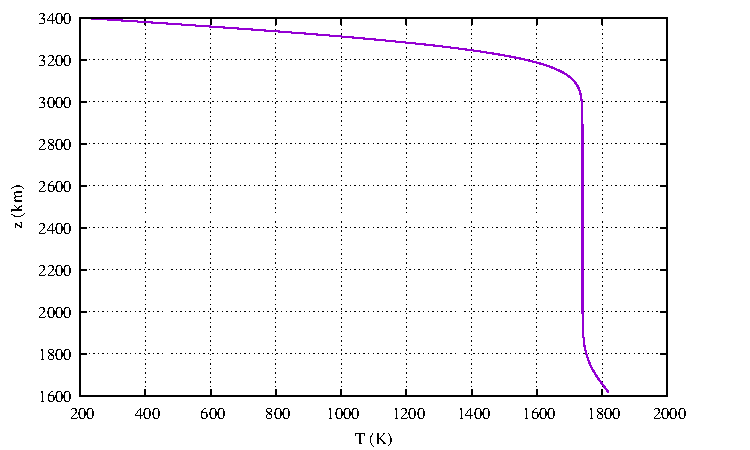
\includegraphics[width=8cm]{python_codes/fieldstone_183/seki14/T.pdf}
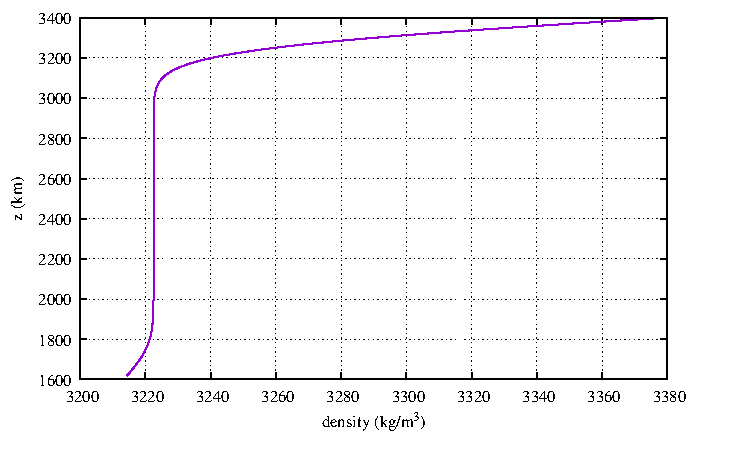
\includegraphics[width=8cm]{python_codes/fieldstone_183/seki14/rho.pdf}\\
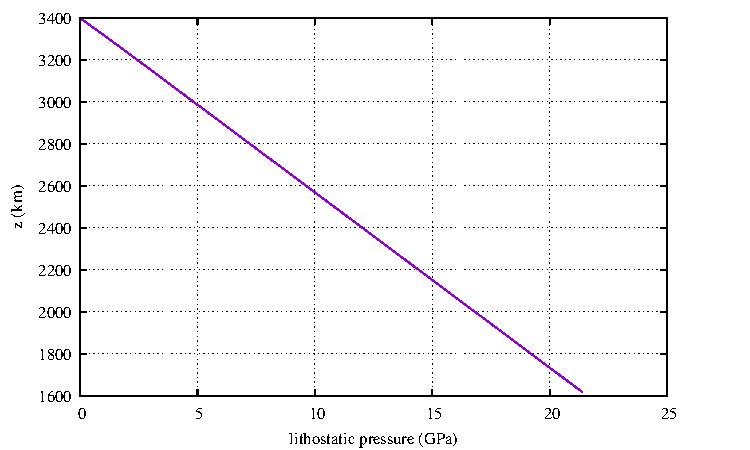
\includegraphics[width=8cm]{python_codes/fieldstone_183/seki14/p.pdf}
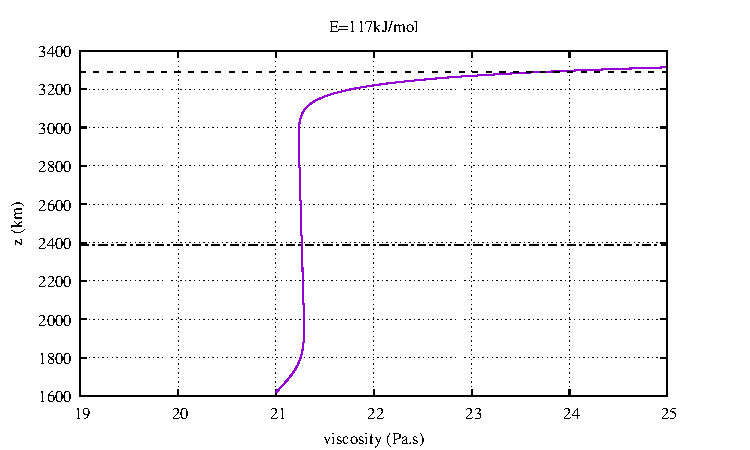
\includegraphics[width=8cm]{python_codes/fieldstone_183/seki14/eta.pdf}
\end{center}



%%%%%%%%%%%%%%%%%%%%%%%%%%%%%%%%%%%%%%
\section*{The Earth a la Coltice et al}

We shall here study 3 articles:
\begin{itemize}
\item \fullcite{arcf18}
\item \fullcite{cohf19}
\item \fullcite{arcf20}
\end{itemize}

%-------------------------------
\subsection*{\textcite{cohf19}}

\begin{displayquote}{\color{darkgray}
To assess how the surface and interior reciprocally drag each other, we
now compute the numerical solution for a more accurate and realistic,
yet challenging, model building upon Arnould et al. \cite{arcf18}. 
All parameters, resulting to a Rayleigh number of $10^7$, are listed in table S1.
Rheology is set with a classic Arrhenius viscosity
\[
\eta(T) \propto \exp \left(
\frac{E_a + p V_a}{RT} - \frac{E_a }{RT_0} 
\right)
\]
where $E_a$ is the activation energy, $V_a$ is the activation volume, 
$R$ is the gas constant, and $p$ is the lithostatic pressure. $T_0$ and 
$\eta_0$ are the reference temperature and viscosity for the Rayleigh number. 
A factor of 30 viscosity jump imposed at the depth of 660 km, and the value of
the yield stress at the surface is 61 MPa.}
\end{displayquote}

We find most of these parameters in table S1 of the paper (see {\tt stone\_cohf19.py}):
\begin{lstlisting}
Rsurf=6371e3
Rcmb=3485e3
rho0=4000
g=9.8
eta0=1e22
V=0.7e-6 #13.8e-6
alpha=3e-5
kappa=1e-6
hcond=3.15
hcapa=hcond/kappa/rho0 ; print('Cp=',hcapa)
Tsurf=255
Tcmb=2645
year=365.25*24*3600
E=160e3
T0=1530 # for viscosity 
\end{lstlisting}

A few remarks:
\begin{itemize}
\item the authors use depth-dependent thermal expansion. We here use
a constant value for simplicity.
\item Tsurf=255K=-18C ??
\item their implicit choice of heat capacity is ...weird: indeed, using $C_p = k/\rho \kappa$
we find $C_p \sim 787$, which is about half what it is in reality.
\item Coltice [personnal communication] indicates that the activation 
volume value in the paper (13.8 cm3/mol) is wrong and should be 0.7cm3/mol instead.
\end{itemize}

Assuming a constant temperature profile $T_m$ in the mantle 
with a half space cooling correction at the surface and the cmb,
we loop over multiple values of Tm, given by 
\begin{lstlisting}
for coeff in (0.5,0.6,0.7,0.8,0.9):
    Tm=(Tcmb-Tsurf)*coeff 
\end{lstlisting}
corresponding to 
Tm=1450.0,
Tm=1689.0,
Tm= 1928.0,
Tm= 2167.0,
Tm= 2406.0.


\begin{center}
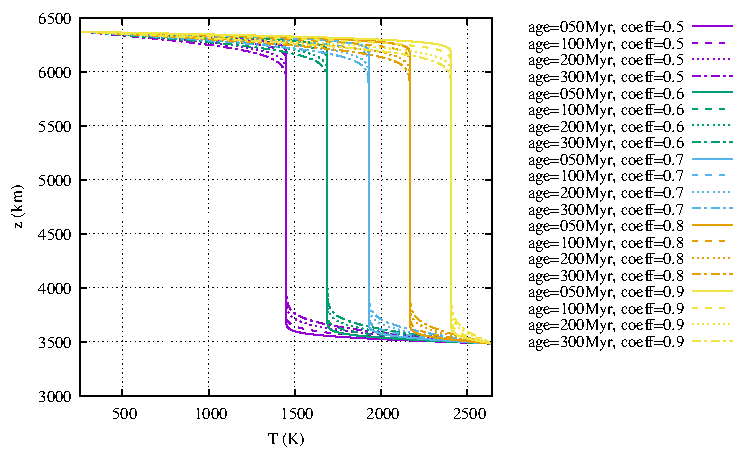
\includegraphics[width=8cm]{python_codes/fieldstone_183/cohf19/T123.pdf}
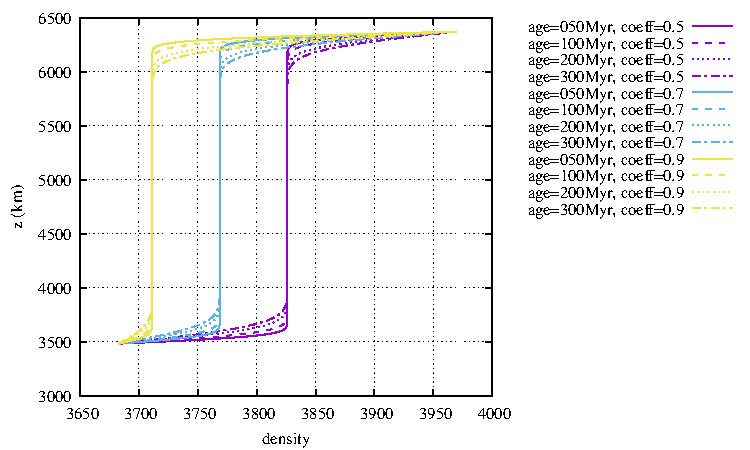
\includegraphics[width=8cm]{python_codes/fieldstone_183/cohf19/rho.pdf} \\
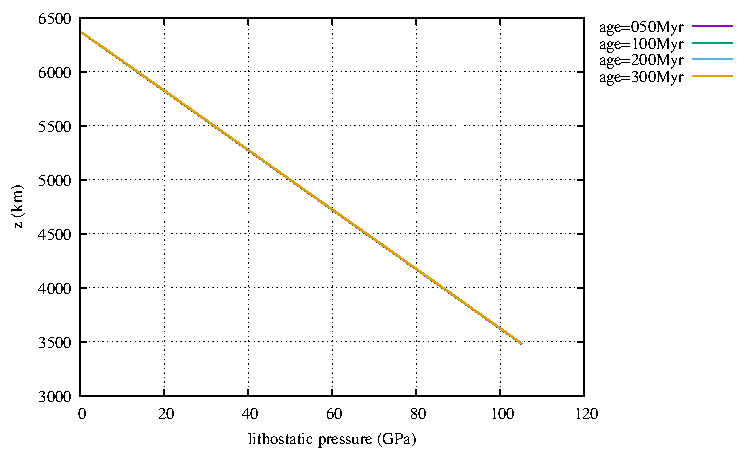
\includegraphics[width=8cm]{python_codes/fieldstone_183/cohf19/p.pdf}
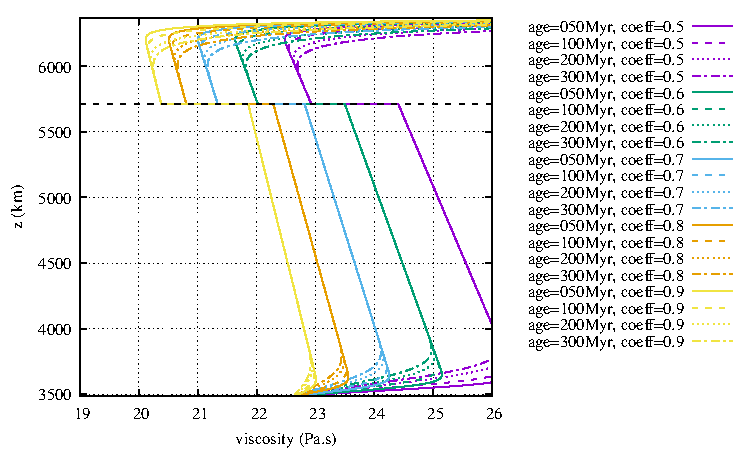
\includegraphics[width=8cm]{python_codes/fieldstone_183/cohf19/eta.pdf}
\end{center}


%-------------------------------
\subsection*{\textcite{arcf18}}

In this article we find (see {\tt stone\_arcf18.py}):
\begin{lstlisting}
Rsurf=6371e3
Rcmb=3485e3
rho0=4400
g=9.8
V=0.7e-6
alpha=3e-5
kappa=1e-6
hcond=3.15
hcapa=hcond/kappa/rho0 ; print('Cp=',hcapa)
Tsurf=255
Tcmb=2390
year=365.25*24*3600
E=142e3
A=-12.5
\end{lstlisting}

with a viscosity given by Eqs. 3\&4:
\[
\eta(z,T)=\eta_0(z) \exp\left(  A + \frac{E_a + p_{lith} V_a}{RT}   \right)
\]
with 
\[
\eta_0(z)=\eta_{ref} \exp \left(
\log 30 \left[ 1 - \frac12 \left( 1 - \tanh \frac{d_0-z}{d_{jump}}   \right)
  \right]
\right)
\]
where $\eta_{ref}$ is the reference nondimensionalized viscosity value 
producing an average value of 1 for $\eta_0(z)$.

Remarks:
\begin{itemize}
\item The $z$-dependency of the rheology of \cite{cohf19} looks a bit different 
than the expression above: in \cite{cohf19} we find $-E/RT_0=160e3/8.34/1530\simeq -12.5$ 
(it is dimensionless) instead of $A$.
We find this value of $A=-12.5$ in Table 1 of \cite{arcf18} in the `nondimensional value' column, 
but we also see $A=-88.75$ in the `dimensional value', which is very weird.
\item The value of $A=-12.5$ is obtained in \cite{cohf19} for $E_a=160kJ/mol$
but in this paper we find $E_a=142kJ/mol$?
\item again the implicit choice of heat capacity is ...weird: indeed, using $C_p = k/\rho \kappa$
we find $C_p \sim 716$, which is about half what it is in reality.
\item in \textcite{arcf20} we find $V=0.44cm3/mol$. Since $V=13.8cm3/mol$
is much too high, we instead here adopt 0.44 instead of 0.7 from Coltice (see above)
\end{itemize}


\begin{center}
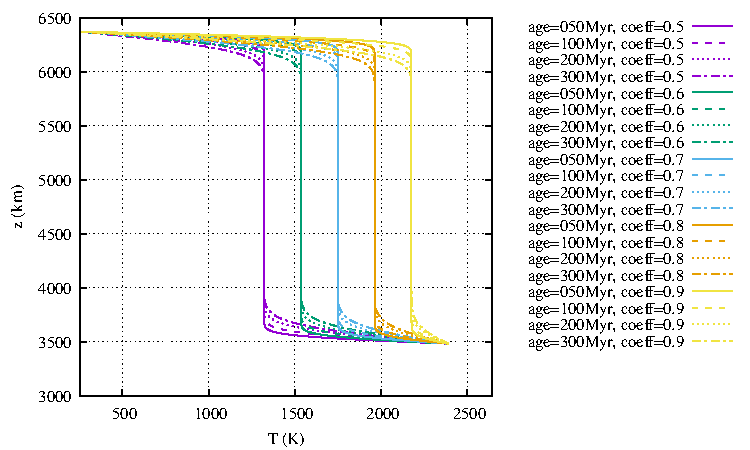
\includegraphics[width=8cm]{python_codes/fieldstone_183/arcf18/T123.pdf}
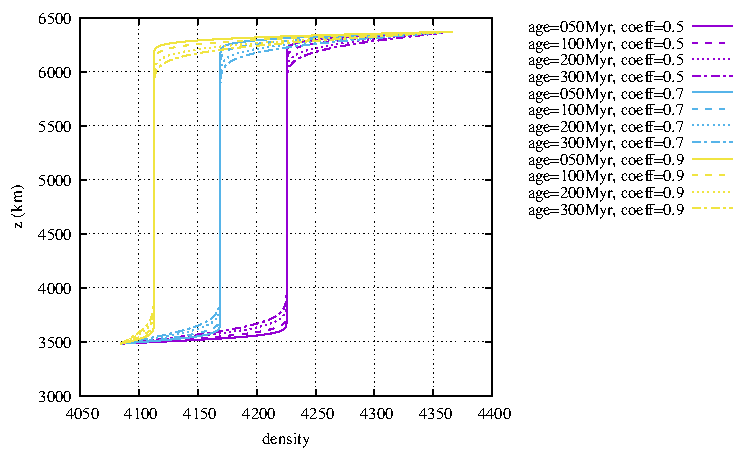
\includegraphics[width=8cm]{python_codes/fieldstone_183/arcf18/rho.pdf} \\
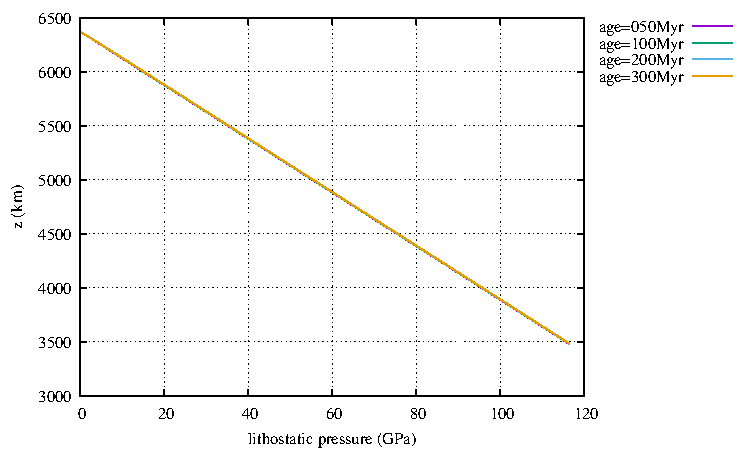
\includegraphics[width=8cm]{python_codes/fieldstone_183/arcf18/p.pdf}
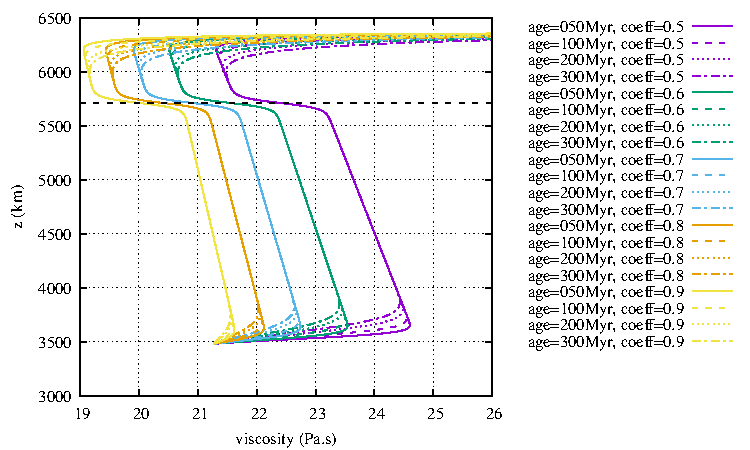
\includegraphics[width=8cm]{python_codes/fieldstone_183/arcf18/eta.pdf}
\end{center}



\newpage

\[
\frac{dT}{dr}= - \frac{\alpha g}{C_p} T
\]
Let us denote $A=\frac{\alpha g}{C_p}$, so that now
\[
\frac{dT}{dr}= - A T
\]
\[
\frac{dT}{T}= - A dr
\]
\[
\int_{T_{pot}}^r \frac{dT}{T} =  - A \int_{R_{surf}}^r dr
\]
\[
\log (T) - \log T_{pot} = -A ( r- R_{surf}  )
\]
\[
\log T = \log (T_{pot})  -A (r- R_{surf} )
\]
\[
T(r) = \exp \left( \log (T_{pot})  -A (r- R_{surf} ) \right)
\]
\[
T(r) = \exp \left( \log (T_{pot}) \right) \exp\left(  -A (r- R_{surf} ) \right)
\]
\[
T(r) = T_{pot} \exp\left(  -A (r- R_{surf} ) \right)
=T_{pot} \exp\left(  - \frac{\alpha g}{C_p} (r- R_{surf} ) \right)
\]

On average in the mantle $\alpha\sim 2\cdot 10^{-5}$, $C_p\sim 1250$ and $g\sim 10$, 
so that $A=\frac{\alpha g}{C_p} \sim 1.6e-7$.






\newpage
%%%%%%%%%%%%%%%%%%%%%%%%%%%%%%%%%%%%%%
\section*{The Earth a la Wang \& Li 2021}

This is based on \fullcite{wali21}.
The setup of the paper is pretty straightforward if not for the usual mix
of dimensioned and dimensionless quantities. 
The parameters are as follows:
\begin{lstlisting}
Rsurf = 6370e3
Rcmb = Rsurf - 1000e3
rho0 = 3300
g = 9.8
eta0 = 1e21
R = 8.314
alpha = 3e-5
kappa = 1e-6
hcapa = 1250
Tsurf = 273
DeltaT = 1350
year = 365.25 * 24 * 3600
\end{lstlisting}

The dimensionless temperature is 0 at the top and 1 at the bottom, while 
the real temperature difference is stated to be 1350C. We then dedude that 
\[
T^\star = \frac{T-T_K}{\Delta T}
\]
where $T_K=273$. We then have $T_{top}=273$ and $T_{bottom}=1350C=1623K$.

The dimensionless viscosity is temperature-dependent and simply given by 
$\eta^\star(T^\star)=\exp (E(1-T^\star))$ with $E=6.91$.
We then have
\begin{eqnarray}
\eta(T) 
&=& \eta_0 \exp \left[ E \left(1 - \frac{T-T_K}{\Delta T} \right)  \right] \nn
\end{eqnarray}

This yields the following temperature and viscosity profiles.

\begin{center}
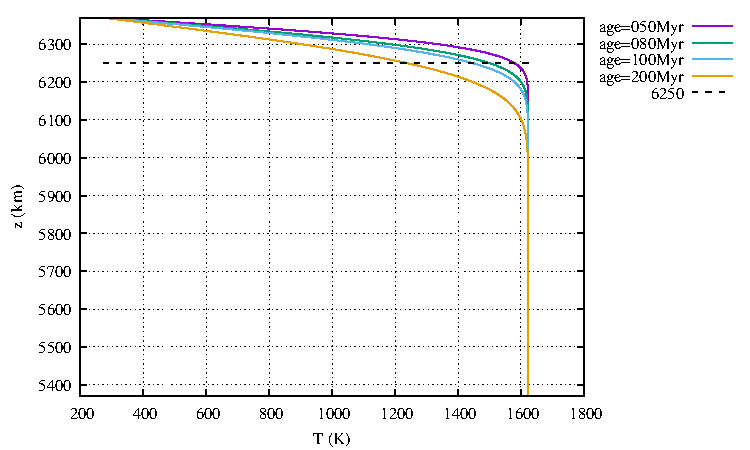
\includegraphics[width=8cm]{python_codes/fieldstone_183/wali21/T.pdf}
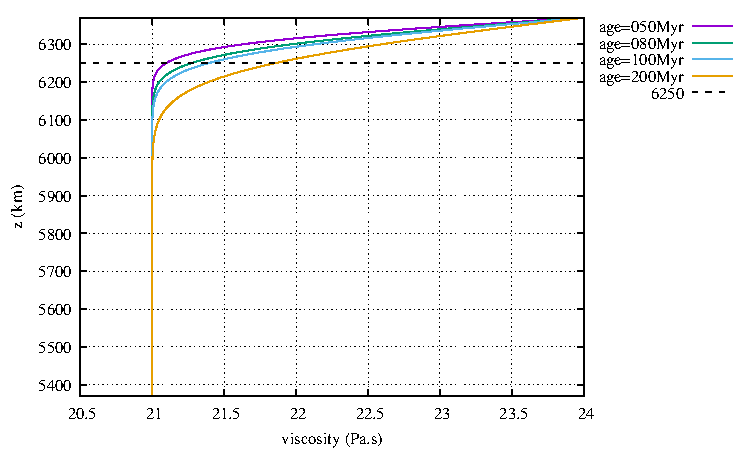
\includegraphics[width=8cm]{python_codes/fieldstone_183/wali21/eta.pdf} 
\end{center}

Unfortunately this viscosity expression cannot be reworked to fit 
existing viscosity forms in ASPECT (dislocation creep, diffusion creep, ...).
This is quite a peculiar choice: using an extremely simplified 
rheology that does not even fit any known deformation mechanism in the Earth
so as to produce a study that focuses on dynamic topography is rather wild, in my 
opinion.

One solution could be to actually use a diffusion creep approach. 
We then set 
\[
\eta(T) = \frac12 A^{-1} \exp \frac{Q}{RT}
\]
We vary Q between 100kJ/mol and 400kJ/mol, and adapt A so that 
the viscosity is at $10^{21}$ in the deeper mantle at $T=T_m$.
We then obtain the following viscosity profiles:

\begin{center}
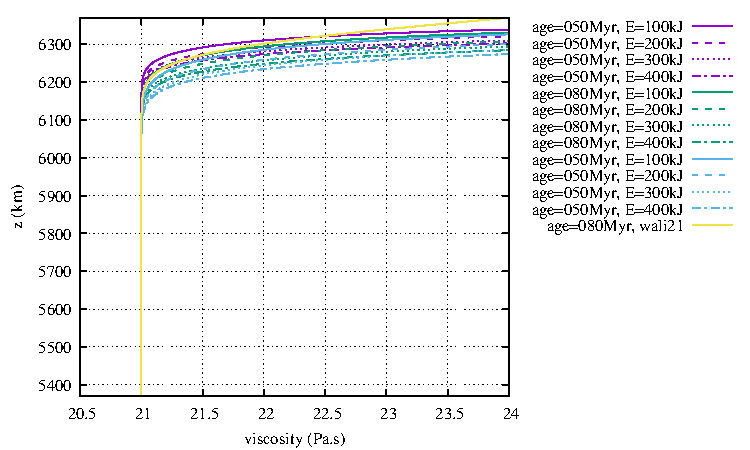
\includegraphics[width=8cm]{python_codes/fieldstone_183/wali21/eta2.pdf} 
\end{center}

It looks like we recover a similar viscosity profile, 
although the viscosity becomes infinite towards the surface so that a 
limiter is then needed.





